\documentclass[twocolumn]{jarticle}

\usepackage[dvipdfmx]{graphicx}
\usepackage{amsmath}
\usepackage{amssymb}
\usepackage{amsfonts}
\usepackage{jsaiac}
\usepackage{array}
\usepackage{multirow}
\usepackage{booktabs}
\usepackage{ascmac}

\usepackage{listings}
\lstdefinestyle{mystyle}{
    basicstyle=\ttfamily\footnotesize,
    stepnumber=1,
    frame=single,
    breaklines=true,
    captionpos=b
}

\def\thline{\noalign{\hrule height 1.3pt}}
\def\tvline{\vrule width 1.3pt}

\title{
\jtitle{
\\BLEを用いた食堂の混雑度センシングに関する研究報告
\\~誰もが不便なく利用できる学食を目指して~
}
}

\jaddress{m807040z@mails.cc.ehime-u.ac.jp}

\author{
\jname{平本宗大 上村航平 大西真輝 佐野一樹 高屋友輔 平木晶 三好涼太 山下智也 吉原駿平}
}

\affiliate{
\jname{理工学研究科 数理情報プログラム}
}

\begin{abstract}
本プロジェクトは,2つの側面を持つプロジェクトである.
1つ目は,学術的な観点からBluetooth Low Energy (BLE)を用いた混雑度推定についての研究を行うことである.
2つ目は,学生食堂において,BLEを用いた混雑度推定システムを実装し,ICT技術を用いて,実際の課題解決を目指すことである.
この2つの側面を一気通貫して1つのプロジェクトとして進める.
我々は,このプロジェクトを通して,学術的な成果を即座に実社会に実装できることを証明した.
このような取り組みを積極的に行うことは,より高度化するICT社会において,
研究から生まれた成果をスピード感をもって社会に還元することに必要不可欠であると考える.
この報告書において,プロジェクトの学術的な側面についてはA-1からA-8,その実装についてはB-1からB-3に分けて報告する.

\end{abstract}

\def\Style{``jsaiac.sty''}
\def\BibTeX{{\rm B\kern-.05em{\sc i\kern-.025em b}\kern-.08em%
 T\kern-.1667em\lower.7ex\hbox{E}\kern-.125emX}}
\def\JBibTeX{\leavevmode\lower .6ex\hbox{J}\kern-0.15em\BibTeX}
\def\LaTeXe{\LaTeX\kern.15em2$_{\textstyle\varepsilon}$}

\begin{document}
\maketitle
  \section*{A-1. はじめに}
\section*{A-2. 関連技術}

\subsection*{2.1 BLE\ (Bluetooth Low Energy)}
BLE(Bluetooth Low Energy)は,Bluetooth規格の一部であり,低消費電力での通信を目的としている\cite{ble}.主にセンサーデバイスやウェアラブル機器,IoTデバイスに利用され,短距離無線通信を効率的に行うことが可能である.従来のBluetooth Classicと比較して消費電力が非常に少なく,バッテリー駆動のデバイスに適している\cite{ble}.また,BLEはAdvertisingとScaningの2つのモードを利用して通信を行う\cite{ble}.Advertisingはデバイスが周期的に信号を送信するモードであり,Scaningは信号を受信し解析するモードである.これにより,BLEは位置情報の測定やデバイスの存在検知に活用されている.

\subsection*{2.2 RSSI(Received Signal Strength Indicator)とMACアドレス}
RSSI(Received Signal Strength Indicator)は,受信信号強度を示す指標であり,無線通信において受信側のデバイスが測定する信号の強度を示す値である\cite{ble}.一般に,RSSIは負のdBm(デシベルミリワット)単位で表され,値が0に近いほど信号が強く,負の値が大きくなるほど信号が弱いことを意味する.

RSSIは,無線通信の品質評価や通信経路の選択,位置推定など,さまざまな用途で利用される.特に位置推定では,複数のアクセスポイントや基地局からのRSSI値を用いて,電波の減衰特性に基づいた推定を行う手法が一般的である.RSSIの測定は追加のハードウェアは必要とせず,ほとんどの無線通信モジュールに標準的に搭載されているため,位置情報の取得においてコスト効率の良い手法とされている.

しかし,RSSIの測定値は周囲の環境要因に大きく影響される\cite{ble}.例えば,電波の反射,回折,散乱,遮蔽物の存在などが測定値に誤差を生じさせる.特に屋内環境ではマルチパス伝播の影響が顕著であり,精度の低下を引き起こす.また,異なるデバイスやチップセットによってRSSIの測定精度や値の補正方法が異なるため,環境に依存しない正確な推定を行うためには,適切なキャリブレーションやフィルタリングが必要となる.


MACアドレス(Media Access Control Address)は,ネットワークインターフェースに一意に割り当てられた識別子であり,ネットワーク層でのデバイス識別や通信制御に用いられる\cite{tanenbaum}.MACアドレスは通常48ビットの長さを持ち,12桁の16進数(例:\texttt{00:1A:2B:3C:4D:5E})で表記される.MACアドレスはOSI参照モデル\cite{tanenbaum}のデータリンク層において使用され,同一ネットワーク内での通信を確立する際の基本的な識別子として機能する.

MACアドレスは物理的にネットワーク機器に埋め込まれており,通常はデバイスの製造時に割り当てられる.最初の24ビットは製造者識別子(Organizationally Unique Identifier, OUI)として定められ,特定のメーカーに割り当てられる.残りの24ビットはメーカーが独自に管理し,各デバイスに一意となるよう設定される.この仕組みにより,世界中の全てのネットワークデバイスに対して一意のMACアドレスを付与することが可能となっている.

\subsection*{2.3 Raspberry Pi 4}
Raspberry Pi 4は,シングルボードコンピュータであり,BLE通信の受信やデータ処理を行うためのデバイスとして利用することができる\cite{rasPi}.ARM Cortex-A72プロセッサと最大8GBのRAMを搭載し,小型ながら高性能な処理が可能である\cite{rasPi}.BLE受信モジュールを搭載しており,周囲のBLEビーコンやデバイスをスキャンして信号強度指標(RSSI)やMACアドレスなどの情報を取得できる\cite{rasPi}.
BLEスキャンは,Raspberry Pi 4に搭載されたBluetooth 5.0対応モジュールを用いて行われる.Linux環境では,hcitoolやbluetoothctlといったコマンドラインツールを使用することで,BLEデバイスを検出し,一定間隔でRSSI値を取得することが可能である.
取得したRSSI値は,距離推定や位置推定の指標として使用される.
また,Raspberry Pi 4は低コストで簡単に配置できるため,複数台を使用した分散型のデータ収集環境を構築することも容易である.各デバイスが収集したデータをネットワークを介して集約・統合し,混雑度推定モデルの入力として利用できる.分散型環境では,各Raspberry Pi 4が独立してデータ収集を行うことで,リアルタイム性を維持しつつ効率的な処理を実現できる.

\subsection*{2.4 回帰モデル}
回帰モデルは,入力変数と出力変数の間の関係を数理的に表現するための統計的手法である\cite{prml}.特にデータの分布や傾向を捉え,未知のデータに対して,ある連続的な目的変数を予測する場合に用いられる.回帰モデルは,データの分布や傾向を捉え,未知のデータに対して予測を行うために用いられる.一般的に,回帰モデルは次の式で表される.

\begin{equation}
	y = f(\mathbf{x}) + \epsilon
\end{equation}
ここで,$y$ は目的変数(従属変数)であり,$\mathbf{x} = (x_1, x_2, \ldots, x_p)$ は $p$ 個の説明変数(独立変数)のベクトルを表す.$f(\mathbf{x})$ は説明変数と目的変数の関係を表す未知の関数であり,$\epsilon$ は誤差項である.誤差項は観測誤差やモデル化の不確実性を表し,通常は平均0,分散$\sigma^2$の正規分布に従うと仮定される.

\subsubsection*{単回帰モデル}
最も基本的な回帰モデルとして,単回帰モデルが挙げられる.単回帰モデルでは,1つの説明変数を用いて目的変数を予測する\cite{prml}.そのモデルは次の式で表される.

\begin{equation}
	y = \beta_0 + \beta_1 x + \epsilon
\end{equation}
ここで,$x$ は説明変数,$y$ は目的変数である.$\beta_0$ は切片(定数項)であり,説明変数が0のときの目的変数の期待値を表す.$\beta_1$ は回帰係数(傾き)で,説明変数が1単位増加したときに目的変数がどの程度変化するかを示す.$\epsilon$ は誤差項であり,観測値とモデルの予測値の差を含む.

\subsubsection*{重回帰モデル}
複数の説明変数を用いる場合,重回帰モデルが使用される\cite{prml}.重回帰モデルは次のように表される.

\begin{equation}
	y = \beta_0 + \beta_1 x_1 + \beta_2 x_2 + \cdots + \beta_p x_p + \epsilon
\end{equation}
ここで,$x_1, x_2, \ldots, x_p$ は $p$ 個の説明変数,$\beta_0$ は切片,$\beta_1, \beta_2, \ldots, \beta_p$ は各説明変数に対する回帰係数である.誤差項 $\epsilon$ は,単回帰モデルと同様に観測誤差やモデル化の不確実性を表す.

\subsubsection*{最小二乗法}
回帰モデルの係数 $\beta_0, \beta_1, \ldots, \beta_p$ を推定するためには,一般に最小二乗法が用いられる\cite{prml}.最小二乗法では,観測値とモデルの予測値の差の二乗和を最小化することを目的とする.損失関数(残差平方和)は次のように定義される.

\begin{equation}
	L(\beta_0, \beta_1, \ldots, \beta_p) = \sum_{i=1}^{n} (y_i - \hat{y}_i)^2 = \sum_{i=1}^{n} (y_i - \beta_0 - \sum_{j=1}^{p} \beta_j x_{ij})^2
\end{equation}
ここで,$n$ はサンプルサイズ,$y_i$ は $i$ 番目の観測値,$\hat{y}_i$ はモデルによって予測された $i$ 番目の値である.$x_{ij}$ は $i$ 番目のサンプルの $j$ 番目の説明変数を示す.損失関数 $L$ を最小化することで,最適な回帰係数を求めることができる.

最小二乗法の解は以下の正規方程式を解くことで得られる.

\begin{equation}
	(\mathbf{X}^T \mathbf{X}) \mathbf{\beta} = \mathbf{X}^T \mathbf{y}
\end{equation}
ここで,$\mathbf{X}$ は $n \times (p+1)$ 次元の説明変数のデザイン行列であり,$\mathbf{\beta}$ は $(p+1)$ 次元の回帰係数のベクトル,$\mathbf{y}$ は $n$ 次元の目的変数のベクトルを表す.$\mathbf{X}^T$ は $\mathbf{X}$ の転置行列である.この方程式を解くことで,最小二乗推定量を得ることができる.

\subsubsection*{SVR(Suuport Vector Regression)}
SVRは,サポートベクターマシン(SVM)の枠組みに基づく回帰手法であり,高次元空間における非線形な関係も捉えることが可能である\cite{prml}.SVRでは,予測値が実際の値からある許容範囲($\epsilon$)以内に収まるような関数を学習する.このとき,モデルの複雑さを抑えるために,関数の平滑性も同時に最適化の対象とする.SVRの回帰関数は,次のように表される.

\begin{equation}
	f(\mathbf{x}) = \langle \mathbf{w}, \phi(\mathbf{x}) \rangle + b
\end{equation}
ここで,$\mathbf{w}$ は重みベクトル,$b$ はバイアス項,$\phi(\mathbf{x})$ は入力ベクトル $\mathbf{x}$ を高次元空間に写像する特徴変換関数である.SVRでは以下の最適化問題を解くことで回帰関数を学習する.

\begin{align}
	\min_{\mathbf{w}, b, \xi_i, \xi_i^*} \quad & \frac{1}{2} \|\mathbf{w}\|^2 + C \sum_{i=1}^{n} (\xi_i + \xi_i^*) \\
	\text{subject to} \quad 
	& y_i - \langle \mathbf{w}, \phi(\mathbf{x}_i) \rangle - b \leq \epsilon + \xi_i \\
	& \langle \mathbf{w}, \phi(\mathbf{x}_i) \rangle + b - y_i \leq \epsilon + \xi_i^* \\
	& \xi_i \geq 0, \quad \xi_i^* \geq 0, \quad i = 1, \ldots, n
\end{align}
ここで,$C$ は誤差に対するペナルティの重みを調整する正則化パラメータであり,大きな値をとると予測誤差に対して厳しくなり,小さな値をとると,
ある程度の誤差を許容するようになる.$\xi_i$ および $\xi_i^*$ は,実際の値と予測値の差が許容範囲 $\epsilon$ を超えた場合に,その超過分を補うために導入される変数(スラック変数)である.このスラック変数の値が$0$であれば,予測誤差は $\epsilon$ の範囲内に収まっていることを意味する.

また,SVRでは入力データを高次元空間に写像して回帰を行うが,このときカーネルトリックと呼ばれる手法を用いることで,変換後の特徴量 $\phi(\mathbf{x})$ を明示的に計算せずに内積の計算が可能となる.これにより,非線形な関係を効率的に捉えることができる.よく使われるカーネル関数には,単純な関係を表す線形カーネル,非線形な関係に対応する多項式カーネル,滑らかで複雑な関係を捉えるのに適したRBF(Radial Basis Function)カーネルなどがある.

\subsection*{2.5 決定木とそのモデル}
決定木は,分類および回帰のための機械学習モデルの一つであり,データを階層的に分割することで予測を行う手法である\cite{prml}.木構造を持つこのモデルは,根ノードから始まり,内部ノードで特徴量に基づいた条件分岐を行い,最終的に葉ノードに到達して予測結果を出力する.

決定木は直感的に理解しやすく,可視化が容易であるため,特徴量の重要度を評価する際にも有用である.特に,非線形な関係や複雑なデータに対しても効果的に学習を行うことができる.

決定木における分割は,各ノードにおいて目的変数と特徴量の関係を最もよく説明できる条件を選択することで行われる.分類問題の場合はジニ不純度 (Gini Impurity) \cite{gini}やエントロピー,回帰問題の場合は分散の減少量が評価基準として用いられる.

例えば,ノード $t$ におけるジニ不純度 $G(t)$ は次の式で表される.

\begin{equation}
	G(t) = 1 - \sum_{k=1}^{K} p_k^2
\end{equation}
ここで,$K$ はクラスの数,$p_k$ はクラス $k$ に属するサンプルの割合を表す.エントロピー$H(t)$は以下のように表される.

\begin{equation}
	H(t) = - \sum_{k=1}^{K} p_k \log p_k
\end{equation}
回帰問題においては,ノード $t$ の分散 $V(t)$ を用いて評価を行う.

\begin{equation}
	V(t) = \frac{1}{N_t} \sum_{i \in t} (y_i - \bar{y}_t)^2
\end{equation}
ここで,$N_t$ はノード $t$ 内のサンプル数,$y_i$ は $i$ 番目の目的変数,$\bar{y}_t$ はノード $t$ の平均値である.


決定木は単体で使用されることも多いが,アンサンブル学習の手法においても重要な役割を果たしている.以下に,決定木と深く関連する手法をいくつか挙げる.


\subsubsection*{Random Forest}
複数の決定木を組み合わせて予測を行う手法である\cite{randomforest}.各決定木は,異なるデータサンプルで学習され,最終的な予測は各木の予測結果の平均または多数決に基づいて行われる.これにより,過学習のリスクを減少させ,高い汎化性能を得ることができる.

\subsubsection*{XGBoost}
予測の誤りを少しずつ修正しながら,複数の決定木を順番に追加していく手法(ブースティング)に基づいている\cite{xgboost}.最初の木でうまく予測できなかった部分を,次の木が重点的に学習するように工夫されている.XGBoostはこのブースティングを効率よく実行するためのアルゴリズムであり,学習の速さと精度の高さから,さまざまな分野で広く使われている.

\subsubsection*{LightGBM}
XGBoostと同様にブースティングの考え方に基づくが,特に大量のデータに対して効率的に学習できるように設計されている\cite{lightgbm}.一般的な方法では,決定木を上から順に分割していくが,LightGBMでは,より精度が高くなるような葉の部分(木の末端)を優先して分割する方法を採用している.これにより,学習時間を短縮しつつ,高い予測性能を実現している.

\subsubsection*{CatBoost}
勾配ブースティング決定木(Gradient Boosting Decision Tree)ベースの機械学習ライブラリである\cite{catboost}.カテゴリデータの処理が得意であり,高精度な予測が可能である.特に欠損値の処理や不均衡データへの対応能力が高いため,BLEのようなノイズの多いデータにも適している.
また,決定木の構築過程でカテゴリカル特徴量を最適にエンコードすることで,予測精度を向上させる.さらに,過学習を抑制する正則化手法や高速な学習アルゴリズムが組み込まれているため,大規模なBLEデータの解析にも適している.

\subsection*{2.6 BLEを用いた人数推定の先行研究}
近年,スマートフォン等のモバイルデバイスが発するBLE信号を利用した混雑度推定の研究が注目されている.松田ら~\cite{senkou}は,空間内に設置したBLEビーコンによって空間内に存在するBLE信号を受信し,その受信状況から公共空間内の混雑度を推定する手法(BLECE: BLE-based Crowdedness Estimation)を提案している.

\subsubsection*{実験対象およびデータ収集環境}

実験は以下の4つの空間で実施された:

\begin{itemize}
  \item 空間A:飲食店(カフェ,約25席,正方形)
  \item 空間B:飲食店(とんかつ店,約50席,正方形)
  \item 空間C:飲食店(とんかつ店,約50席,長方形)
  \item 空間D:公共施設(市立図書館,L字形,定員不定)
\end{itemize}

各空間には,BLECEノード(Raspberry Pi 4 Model B + BUFFALO製BLEドングル + LTEドングル)を1〜3台設置し,15秒間隔(スキャン10秒+スリープ5秒)でBLEスキャンを実施された.スキャンにより取得されたデータは,BDアドレス(Bluetooth Device Address)およびRSSIを含むものであり,モバイル回線を通じてクラウドに送信・保存された.

混雑度の正解データは以下の方法で取得された:

\begin{itemize}
  \item 空間A〜C:出入口に設置した俯瞰カメラによる映像を基に5分ごとで人数を計測
  \item 空間D:調査員による15分ごとの目視計測
\end{itemize}

\subsubsection*{データ処理と特徴量設計}

BLECEノードのスキャン結果は非同期であるため,時刻を基準に直近のスキャン結果を統合し,BLEノード数に依存しない仮想的な1点のデータとして扱う.複数ノードにより同一BDアドレスが観測された場合は,最もRSSIが強い(=距離が近いと想定される)値を採用する.

特徴量は,空間内におけるBLE信号の統計的な変動,および時間帯による人流の傾向を捉えることを目的として設計されている.主な特徴量は表\ref{tbl:blece_features}に示す.

\begin{table}[tb]
	\centering
	\caption{先行研究で使用された特徴量一覧}
	\label{tbl:blece_features}
	\small
	\doublerulesep=0.3pt
    \begin{tabular}{l|p{5cm}} \hline\hline\hline
		特徴量名 & 内容 \\ \hline
		all\_num\_T\textsubscript{sec} & 過去 $T$ 秒間にスキャンされた,BD アドレスの総数\\ \hline
    unique\_num\_T\textsubscript{sec} & 過去 $T$ 秒間にスキャンされた,BD アドレスのユニーク数 \\ \hline
    unique\_ratio\_T\textsubscript{sec} & 過去 $T$ 秒間にスキャンされた,BD アドレスのうち,ユニークなデバイスの占める割合(ユニーク数 / 総数) \\ \hline
    unique\_num\_T\textsubscript{sec}\_Sdb & 過去 $T$ 秒間にスキャンされた,BD アドレスのうち,RSSI が閾値 Sdb より大きいもののユニーク数 \\ \hline\hline\hline
	\end{tabular}
\end{table}

ここで,$T$は過去の参照時間(15, 30, 45, 60秒),$S$はRSSIの閾値(--60〜--90\,dB,5\,dB刻み)であり,複数パターンを組み合わせて複数の特徴量を生成している.これにより,デバイスを所持した人の出入りや信号の断続的な観測によるノイズを軽減しつつ,空間内の人数変動を統計的に捉えることを可能にしている.

\subsubsection*{モデル構築と評価}

混雑度推定には,以下の3つの回帰モデルが用いられた:

\begin{itemize}
  \item Support Vector Regressor(SVR)
  \item Random Forest Regressor(RFR)
  \item XGBoost Regressor(XGBR)
\end{itemize}

各モデルのハイパーパラメータはGridSearchCVにより最適化され,3分割交差検証によって評価された.評価指標には以下の3種が用いられている:

\begin{itemize}
  \item 平均絶対誤差(MAE: Mean Absolute Error)
  \item 平均絶対パーセント誤差(MAPE: Mean Absolute Percentage Error)
  \item 二乗平均平方根誤差(RMSE: Root Mean Squared Error)
\end{itemize}

実験の結果,XGBRは全体的に最も良好な性能を示し,最大でMAE 4.59人,MAPE 58.1\%,RMSE 5.94人を記録した.特に,ユニークアドレス数やRSSIの強い信号に注目した特徴量(例:\texttt{unique\_num\_30sec\_70db})がモデルの予測性能に大きく寄与していることが,特徴量重要度の分析から示されていた.

\section*{A-3. データ収集から特徴量抽出}
この章では,BLEを用いた混雑度推定手法について述べる.

\subsection*{3.1 BLEスキャンと正解ラベルの取得}
この章では,学生食堂内のBLEデータと,その時点の食堂利用人数の計測方法を述べる.

\subsubsection*{Raspberry PiによるBLEスキャン}
BLEスキャンは図\ref{raspi}のようなRaspberry Piを用いて行う.
スキャンは約10秒の間隔で行われ,1回のスキャンに含まれる情報は以下の通りである.
\begin{itemize}
  \item BLE情報(MACアドレス,RSSI)
  \item スキャン時刻
\end{itemize}

\begin{figure}[pt]
  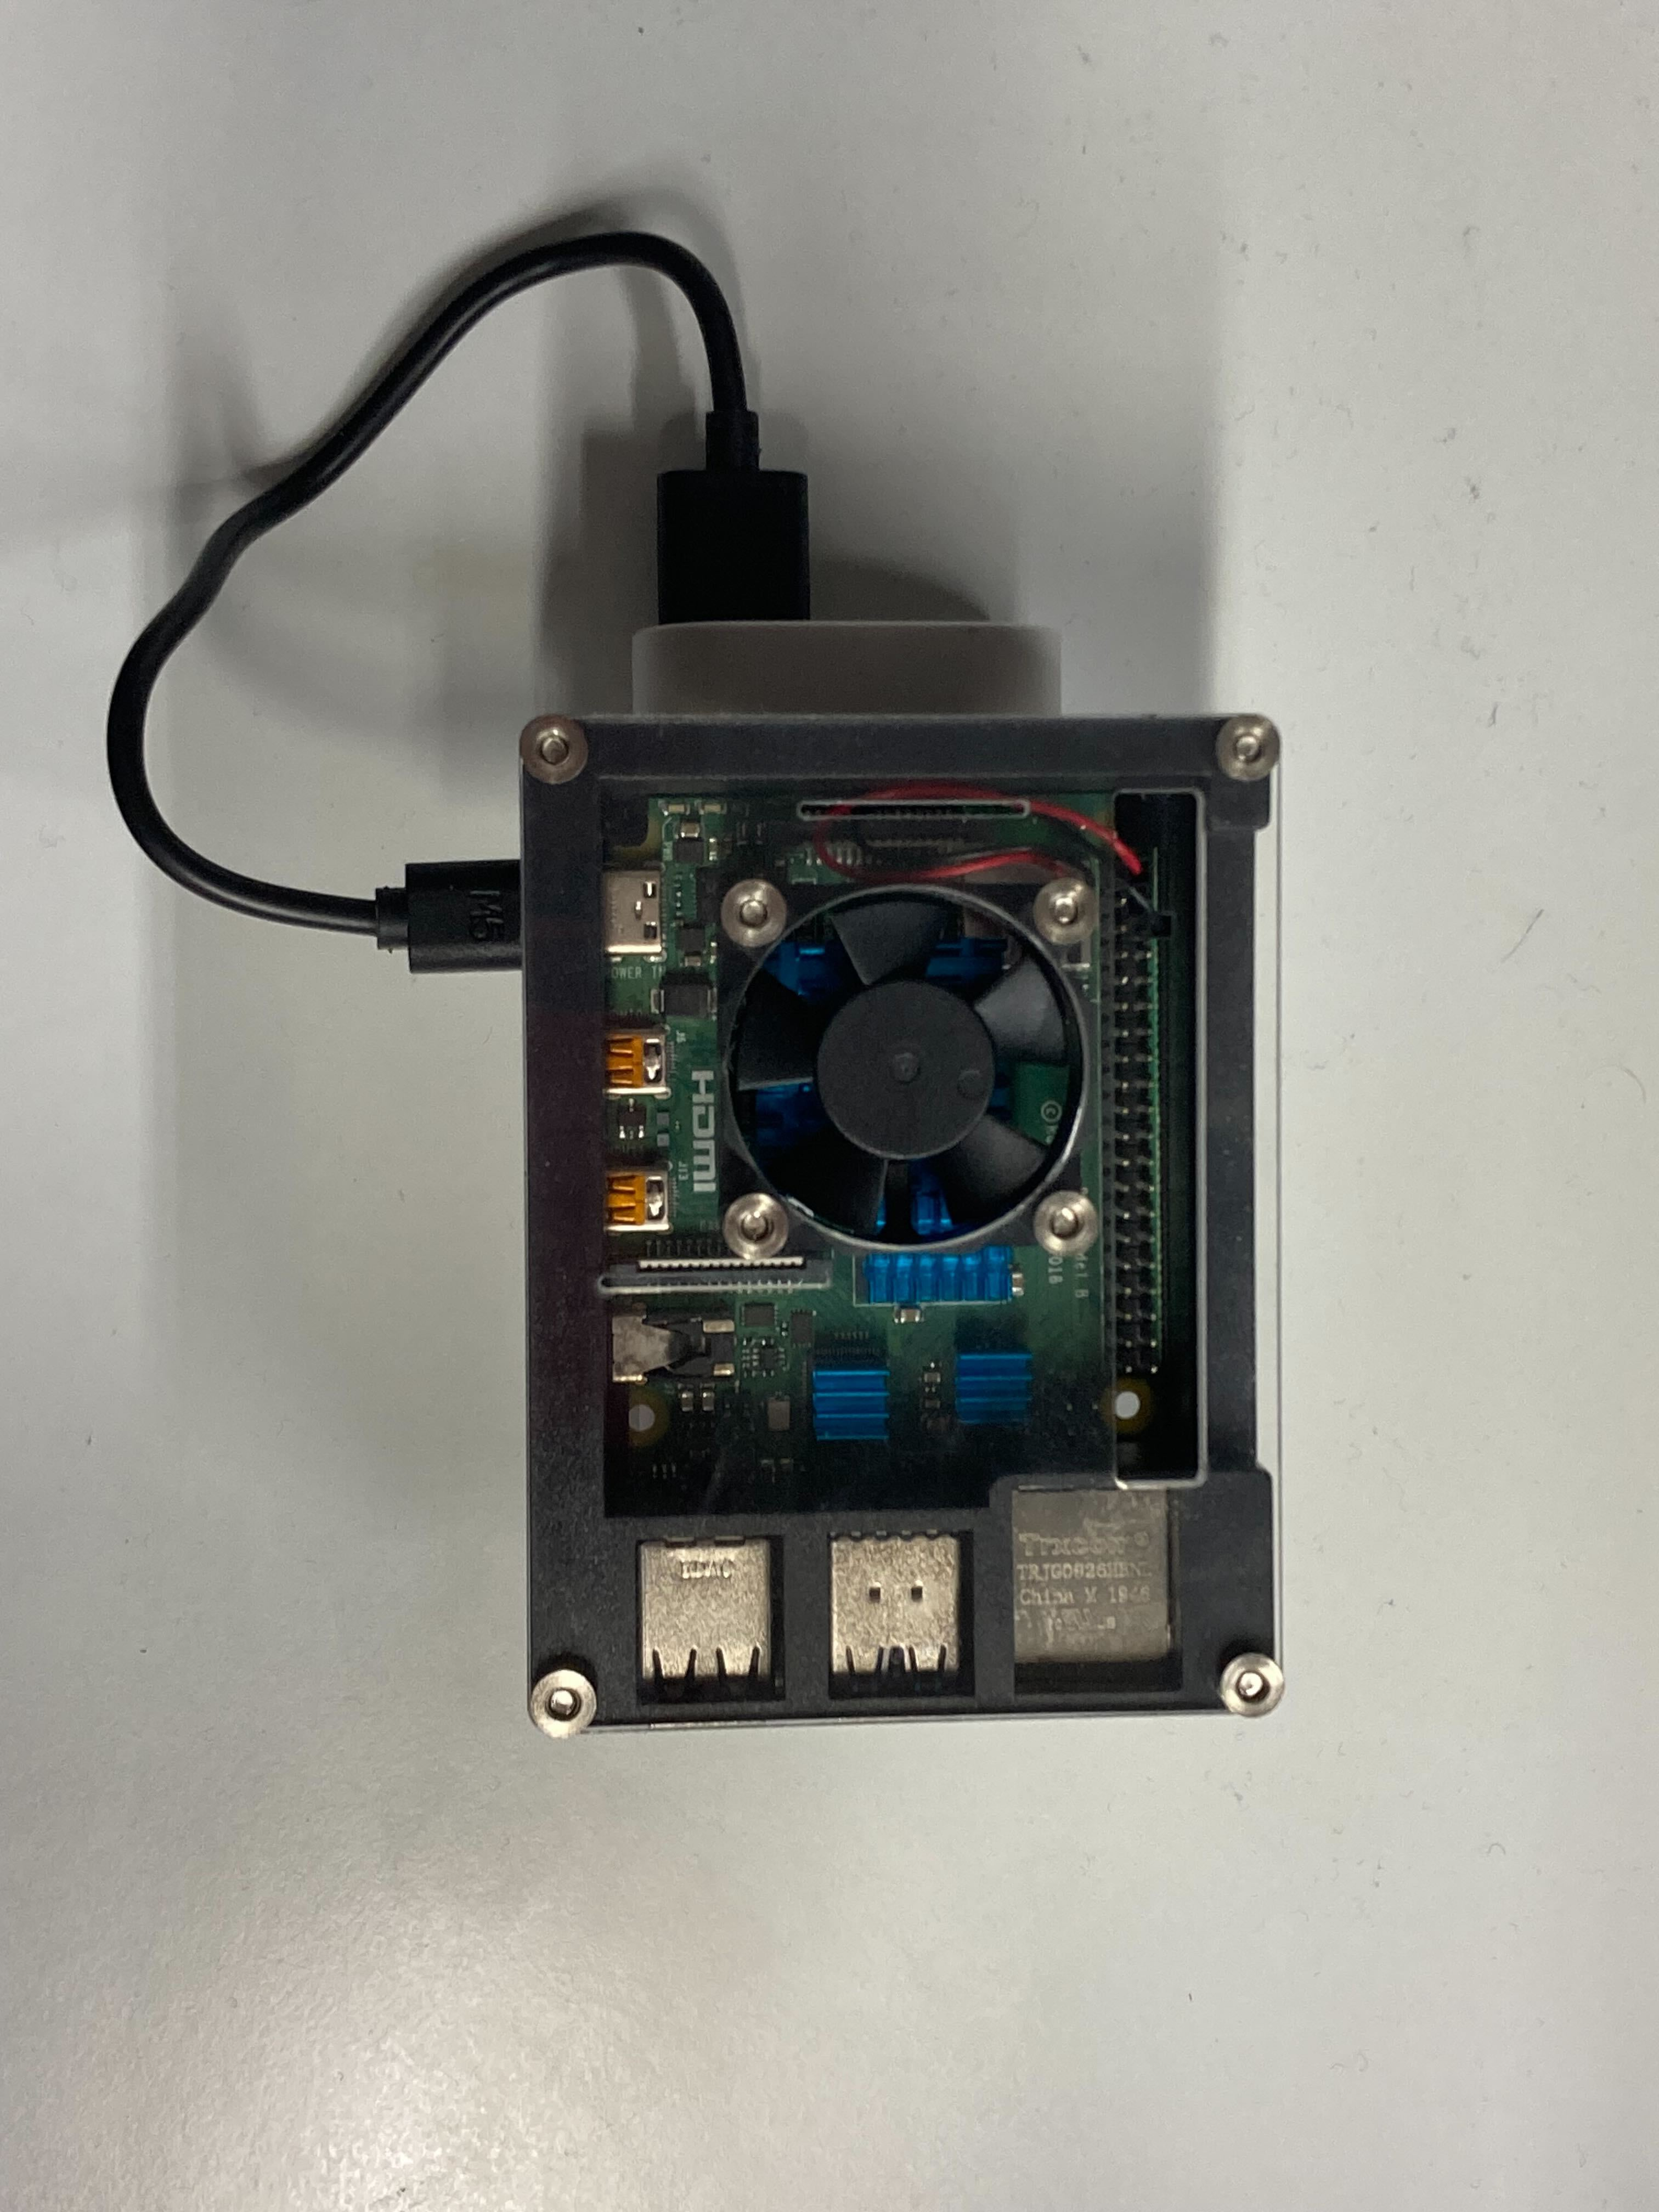
\includegraphics[scale=0.07]{./images/raspi.jpg}
  \centering
  \caption{設置したRaspberry Pi\label{raspi}}
\end{figure}

図\ref{raspi_place}に学生食堂の概略図とRaspberry Piの設置位置を示す.
基本的に壁などの空間を隔てるような障害物は存在せず,開けた空間となっており,そこに机や椅子が配置されている.
Raspberry Piは学生食堂1階と2階それぞれのフロアの中央に計2台配置する.
それぞれのRaspberry Piはお互いに異なるタイミングでスキャンを開始するため,
2台のRaspberry Piは同期していない.
Raspberry Piは1階と2階に配置するが,1階と2階は完全に別の空間ではなく,
スキャン範囲が重複していることに注意が必要である.
\begin{figure}[pt]
  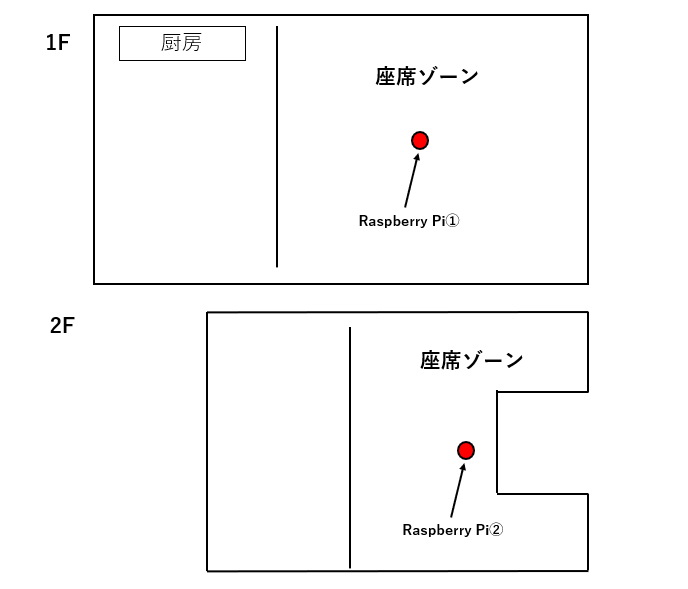
\includegraphics[scale=0.4]{./images/raspi_place.png}
  \centering
  \caption{学生食堂の概略図とRaspberry Piの設置位置\label{raspi_place}}
\end{figure}

\subsubsection*{食堂利用人数の計測}
学生食堂の利用人数は,愛媛大学生協の方に提供していただいた決済データの時間情報と,
利用者が食堂を退出する際に返却されるトレーの数を計測し,算出する.
トレーの数の計測は2人体制で行い,返却場所にカメラを設置する.
計測者間で大きくズレが発生している場合は,カメラを確認し,再度計測する.
決済データは1分間隔で提供されるため,BLEスキャンデータと同様に1分間隔で食堂利用人数を算出する.

\subsection*{3.2 特徴量抽出}
本プロジェクトでは,BLEスキャン情報から混雑度推定に有用な特徴量を抽出し,
モデルに入力することで混雑度を推定する.
基本的な特徴量は松田らの研究\cite{senkou}に基づき,表\ref{tbl:feastures}のように設計した.
unique\_num\_60\textsubscript{sec}\_$S$dbは,
RSSIの値$S$を閾値として,-60から-100まで,10ずつ変化させ,5つ特徴量を得る.
本プロジェクトでは,比較的大規模で開けた空間での混雑度推定を行う.
そのため障害物等による影響が少なく,RSSI値が比較的安定する.
そのためunique\_num\_60\textsubscript{sec}\_$S$dbのような特徴量を用いることで,
より安定した混雑度推定が可能になると考えられる.


\begin{table}[tb]
	\centering
	\caption{特徴量一覧}
	\label{tbl:feastures}
	\small
	\doublerulesep=0.3pt
    \begin{tabular}{l|p{5cm}} \hline\hline\hline
		特徴量名 & 内容 \\ \hline
		all\_num\_T\textsubscript{sec} & 過去 $T$ 秒間にスキャンされた,BD アドレスの総数\\ \hline
    unique\_num\_T\textsubscript{sec} & 過去 $T$ 秒間にスキャンされた,BD アドレスのユニーク数 \\ \hline
    unique\_ratio\_T\textsubscript{sec} & 過去 $T$ 秒間にスキャンされた,BD アドレスのうち,ユニークなデバイスの占める割合(ユニーク数 / 総数) \\ \hline
    unique\_num\_T\textsubscript{sec}\_$S$db & 過去 $T$ 秒間にスキャンされた,BD アドレスのうち,RSSI が閾値 Sdb より大きいもののユニーク数 \\ \hline\hline\hline
	\end{tabular}
\end{table}

\subsection*{3.3 混雑度推定モデル}
混雑度推定モデルは,BLEスキャン情報から抽出した特徴量を入力として,人数を出力するモデルである.
2.4節,2.5節で述べたモデルを用い,人数推定モデルを構築する.
詳しい学習の方法などは,A-4節で述べる.

\subsection*{3.4 評価指標}
本プロジェクトでモデルの性能評価に用いる指標について以下に述べる.

\subsubsection*{平均二乗誤差(Mean Squared Error, MSE)}
MSEは,予測値と実測値の差の二乗の平均を計算することにより,
モデルの誤差を定量化する指標である.数式で表すと,以下のようになる.
\begin{equation}
  \label{eq:mse}
  \mathrm{MSE} = \frac{1}{n} \sum_{i=1}^{n} (y_i - \hat{y}_i)^2
\end{equation}
ここで,$n$はサンプル数,$y_i$は実測値,$\hat{y}_i$は予測値である.
数値が低いほどモデルの性能が良いことを示す.
MSEは,誤差の二乗を取るため,外れ値が大きく影響する.

\subsubsection*{平均絶対誤差(Mean Absolute Error, MAE)}
MAEは,予測値と実測値の差の絶対値の平均を計算することにより,
モデルの誤差を定量化する指標である.数式で表すと,以下のようになる.
\begin{equation}
  \label{eq:mae}
  \mathrm{MAE} = \frac{1}{n} \sum_{i=1}^{n} |y_i - \hat{y}_i|
\end{equation}
ここで,$n$はサンプル数,$y_i$は実測値,$\hat{y}_i$は予測値である.
数値が低いほどモデルの性能が良いことを示す.
MAEは,MSEと比較して,外れ値の影響を受けにくい.

\subsubsection*{決定係数(Coefficient of Determination, $R^2$)}
決定係数は,予測値が実測値をどの程度説明できるかを示す指標である.  
数式で表すと,以下のようになる.
\begin{equation}
  \label{eq:r2}
  R^2 = 1 - \frac{\sum_{i=1}^{n} (y_i - \hat{y}_i)^2}{\sum_{i=1}^{n} (y_i - \bar{y})^2}
\end{equation}
ここで,$n$はサンプル数,$y_i$は実測値,$\hat{y}_i$は予測値,$\bar{y}$は実測値の平均である.
$R^2$の値は$0$から$1$の範囲を取り,$1$に近いほどモデルの性能が良いことを示す.
$R^2$は,モデルの説明力を示す指標であり,$0$に近い場合はモデルが実測値をほとんど説明できていないことを示す.
\section*{A-4. 実験}
本章では,結果と考察について述べる.5.1節で結果について述べ,5.2節で考察について述べる.

\section*{A-6. 結果}

\subsection*{6.1 モデル性能に関する結果}
本項では,5種類の回帰モデル(SVR, RandomForest, XGBoost, LightGBM, CatBoost)に対する性能評価結果を示す.まず,各モデルにおけるデフォルトのパラメータでの実験結果を表\ref{tab:default_results}に示す.次に,Optuna を用いて調整した各モデルの最適なハイパーパラメータを表\ref{tab:best_params}に示す.最後に,パラメータ調整後の各モデルの性能を表\ref{tab:tuned_results}に示す.
\begin{table}[htbp]
    \centering
    \caption{デフォルトパラメータでのモデル評価結果}
    \label{tab:default_results}
    \begin{tabular}{l|p{0.8cm}p{0.8cm}p{0.8cm}|p{0.8cm}p{0.8cm}p{0.8cm}}
        \hline\hline\hline
        モデル & \multicolumn{3}{c|}{検証データ} & \multicolumn{3}{c}{テストデータ} \\
               & MSE & MAE & $R^2$ & MSE & MAE & $R^2$ \\
        \hline
        SVR       & 4042.62 & 41.93 & 0.584 & 4098.13 & 43.35 & 0.585 \\
        RFR       & 525.61  & 15.79 & 0.946 & 550.68  & 15.50 & 0.944 \\
        XGBR      & 547.63  & 15.01 & 0.944 & 618.45  & 15.21 & 0.937 \\
        LGBM      & 456.59  & 14.82 & 0.953 & 487.50  & 14.25 & 0.951 \\
        CatBoost  & 361.71  & 13.30 & 0.963 & 469.74  & 13.67 & 0.952 \\
        \hline\hline\hline
    \end{tabular}
\end{table}

\begin{table}[htbp]
    \centering
    \caption{各モデルの最適パラメータ}
    \label{tab:best_params}
    \begin{tabular}{l|c}
        \hline\hline\hline
        モデル & 最適パラメータ \\
        \hline
        SVR & $C=0.093$ \\ 
            & $\epsilon=0.090$\\
            & $\text{kernel}=\text{linear}$ \\
        \hline
        RandomForest & $\text{max\_depth}=10$ \\
                     & $\text{min\_samples\_split}=2$ \\
                     & $\text{n\_estimators}=4000$ \\
        \hline
        XGBoost & $\text{learning\_rate}=0.082$ \\
                & $\text{max\_depth}=3$ \\
                & $\text{n\_estimators}=4000$ \\
        \hline
        LGBM & $\text{learning\_rate}=0.010$ \\ 
             & $\text{max\_leaves}=63$ \\
             & $\text{n\_estimators}=5000$ \\
        \hline
        CatBoost & $\text{learning\_rate}=0.050$ \\
                 & $\text{max\_depth}=6$ \\
                 & $\text{n\_estimators}=4000$ \\
        \hline\hline\hline
    \end{tabular}
\end{table}

\begin{table}[htbp]
    \centering
    \caption{パラメータ調整後のモデル評価結果}
    \label{tab:tuned_results}
    \begin{tabular}{l|p{0.8cm}p{0.8cm}p{0.8cm}|p{0.8cm}p{0.8cm}p{0.8cm}}
        \hline\hline\hline
        モデル & \multicolumn{3}{c|}{検証データ} & \multicolumn{3}{c}{テストデータ} \\
               & MSE & MAE & $R^2$ & MSE & MAE & $R^2$ \\
        \hline
        SVR       & 1096.46 & 23.31 & 0.887 & 1059.67 & 22.73 & 0.893 \\
        RFR       & 517.24  & 15.84 & 0.947 & 559.44  & 15.66 & 0.943 \\
        XGBR      & 357.44  & 13.35 & 0.963 & 529.44  & 14.51 & 0.946 \\
        LGBM      & 388.36  & 14.03 & 0.960 & 478.33  & 13.71 & 0.952 \\
        CatBoost  & 312.33  & 12.07 & 0.968 & 466.06  & 13.43 & 0.953 \\
        \hline\hline\hline
    \end{tabular}
\end{table}

表\ref{tab:default_results}の結果より,デフォルトのパラメータ設定ではテストデータに対してCatBoostが最も高い$R^2$(0.952)を示し,最も低いMSEおよびMAEを記録した.SVRは$R^2$が0.585と低く,他の手法と比較して精度が劣ることが分かった.XGBoost,LightGBM,RandomForestは$R^2$が0.93以上を達成し,いずれも高い精度を示したが,CatBoostには及ばなかった.

表\ref{tab:tuned_results}の結果より,Optunaによるハイパーパラメータの調整後,全モデルにおいて$R^2$が向上した.SVRは$R^2$が0.893まで改善し,MSEおよびMAEも大幅に低下した.XGBoostとLightGBMは検証データに対する$R^2$がそれぞれ0.963および0.960に向上し,CatBoostは$R^2$が0.968となった.テストデータに対する$R^2$は,調整後のCatBoostが0.953と最も高く,MSEおよびMAEも最も低かった.XGBoostは $R^2$が0.937から0.946へ向上し,LightGBMは0.001ポイント向上した.RandomForestは,$R^2$が0.944から0.943とわずかに低下したが,安定した性能を示した.

\subsection*{6.2 特徴量重要度の分析}
本研究では,最も高い性能を示したCatBoostについて,特徴量の重要度を分析した.特徴量の重要度は,ハイパーパラメータ調整後のCatBoostモデルを用いて算出した.その結果を図\ref{fig:feature_importance} に示す.
\begin{figure}[htbp]
    \centering
    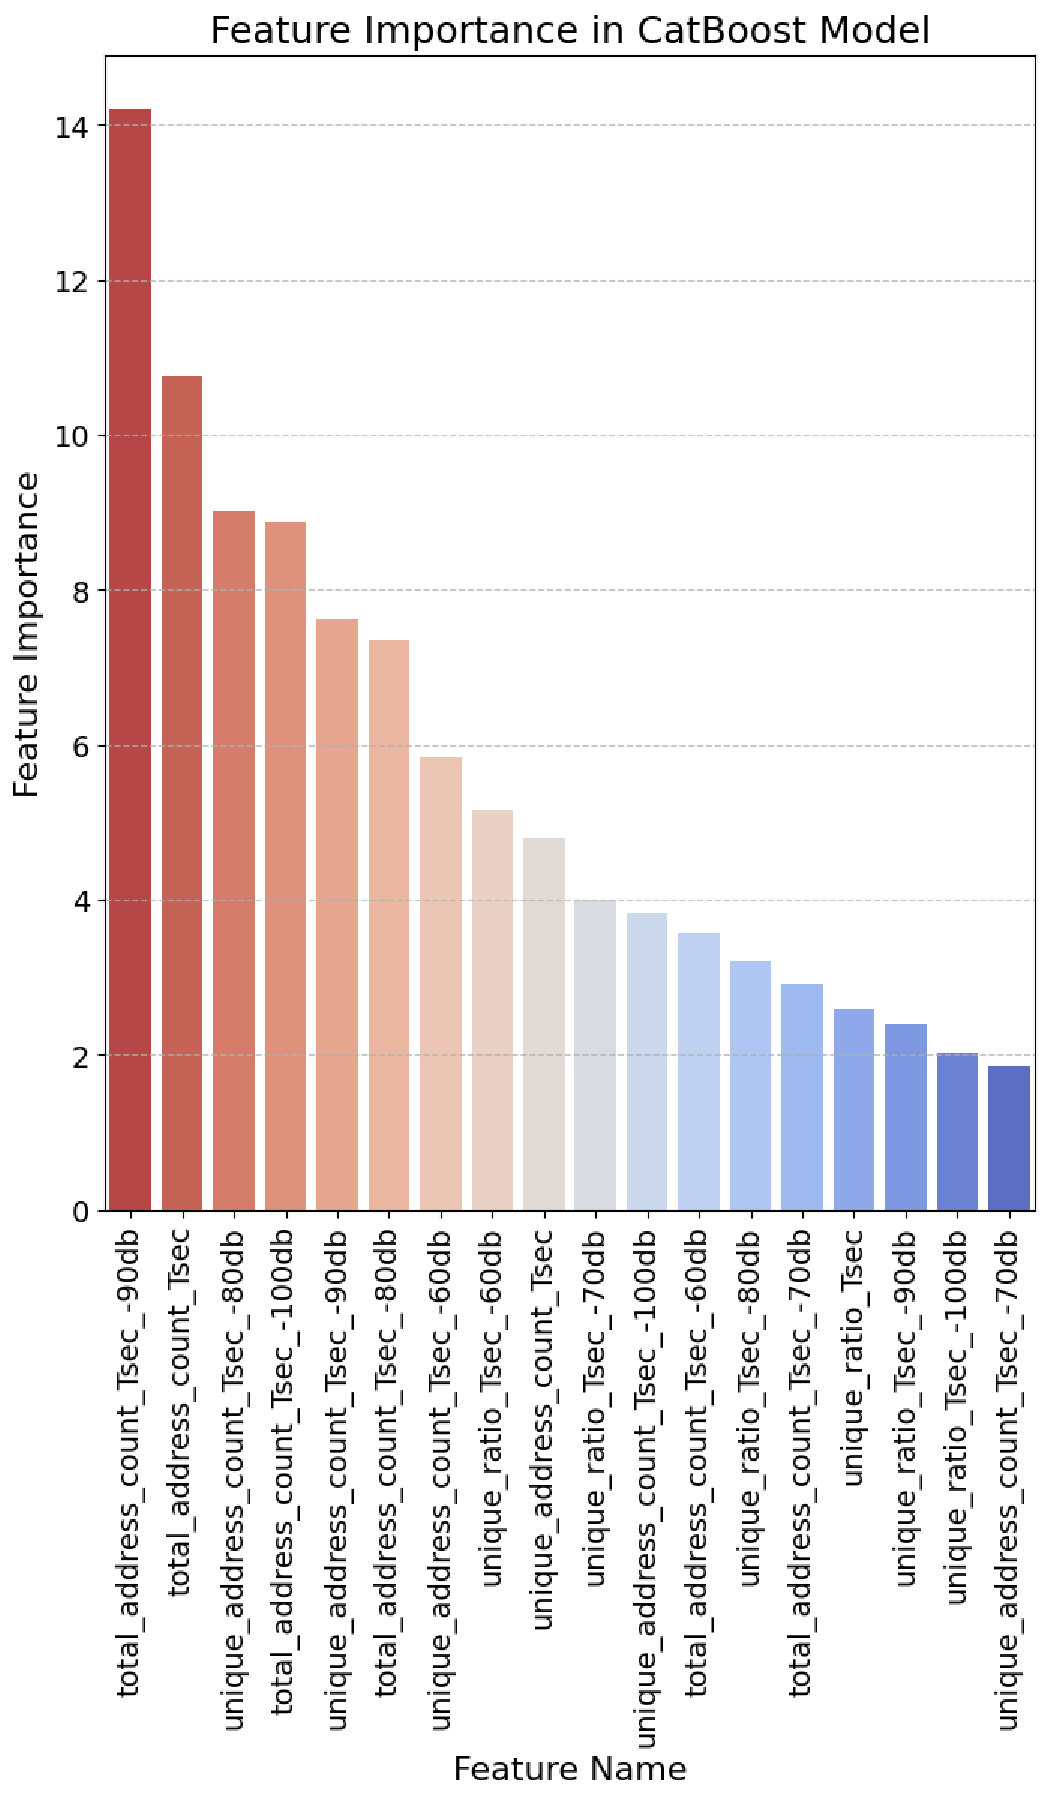
\includegraphics[width=1.2\linewidth]{./fig/feature_importance.pdf}
    \caption{CatBoost における特徴量重要度}
    \label{fig:feature_importance}
\end{figure}

\section*{A-7. 考察}
表\ref{tab:default_results}に示したデフォルトパラメータでの結果を見ると,全体的にCatBoostが最も高い性能を示し,MSEや$R^2$の観点から他のモデルよりも優れていることが分かる.特に,SVRは$R^2$が0.585と低く,MSEやMAEも他の手法と比べて大きいため,本研究に使用するモデルとしては適していない可能性がある.次に,表\ref{tab:best_params}に示したOptunaによるハイパーパラメータ調整を行った結果,表\ref{tab:tuned_results}が示すように,すべてのモデルで性能が向上した.特に,SVRではMSEが約62\%低下し,$R^2$も0.893まで改善された.しかし,それでも他の手法と比較すると誤差が大きく,最適なモデルとは言い難い.XGBoostとLightGBMは調整後に$R^2$がそれぞれ0.946,0.952に向上し,誤差も減少した.また,RandomForestはテストデータにおいて$R^2$が0.944から0.943へわずかに低下したものの,大きな変動はなく安定した性能を示した.

以上の結果を踏まえると,本研究における最適なモデルとしては,CatBoostが有力であると考えられる.MSE,MAE,$R^2$のすべての指標で他のモデルを上回る結果を示しており,特にテストデータに対する汎化性能が優れている.ただし,計算コストやモデルの解釈性を考慮すると,RandomForestやLightGBMも実用的な選択肢となる可能性がある.

\section*{A-8. まとめ}

本研究では,BLEビーコンを活用し,機械学習を用いた学生食堂の混雑度推定手法を提案した.本手法は,Raspberry Piによって収集されたBLEスキャンデータから得られるMACアドレス数やRSSIなどの特徴量を用いて,食堂内の在席人数を回帰的に推定した.

評価においては,実際の食堂環境で時間帯ごとの実測人数とBLEデータを収集し,SVR,Random Forest,XGBoost,LightGBM,CatBoostの5種類の機械学習アルゴリズムにより回帰モデルを構築した.ハイパーパラメータの調整にはOptunaを用いたベイズ最適化を適用し,汎化性能の最大化を図った.

その結果,CatBoostが最も高い決定係数$R^2$を示し,MSEおよびMAEにおいても他モデルと比較して優れた推定精度を示した.また,特徴量の重要度分析から,RSSIに閾値処理を施した特徴量が推定において特に高い寄与を示した.これは,対象とした学生食堂が壁や障害物の少ない開放的な空間であり,BLE信号のRSSIが安定して取得できる環境にあったことが要因と考えられる.これはRSSIの値が利用者数に主に依存し,他の環境要因の影響を受けにくかったため,混雑状況を反映する指標として有効に機能したと考えられる.

さらに,本研究の提案手法はBLEビーコンの配置やデバイスの設置が比較的容易であり,既存の通信インフラに依存せずに導入可能であるため,実環境への応用可能性が高いと考えられる.一方で,デバイス間の信号干渉や,人の移動によるRSSIの変動といった要因が推定精度に与える影響があるため,今後はより堅牢な推定モデルの構築と,長期間にわたるデータの収集・分析を通じた精度向上が課題として挙げられる.

今後の展望としては,他のセンサーデバイスとのデータ融合によるマルチモーダルな混雑推定の実現が挙げられる.

  \section*{B-1. IoTデバイスとAIを用いた課題解決}
\subsection*{1. 混雑度推定の意義}
近年,IoT(Internet of Things)技術の普及が急速に進み,
身の回りの様々なものがインターネットに接続され,情報収集と活用が可能となっている.
さらに,AI(人工知能)技術の飛躍的な進歩により,収集された大量のデータを迅速かつ高度に解析することが可能となった.
IoTデバイスは,人間が直接把握することが難しいリアルタイムの情報を客観的かつ継続的に収集することが可能であり,
AIがその情報を即座に分析し,的確な予測や判断を支援することにより,社会の多様な課題解決に有効な手段として期待されている.

特に,都市部や公共施設での「混雑度推定」は,その利便性と安全性の観点から非常に有意義である.
例えば,近年の新型コロナウイルス感染症のパンデミックにおいては,施設や公共交通機関の混雑状況をリアルタイムで把握し,
混雑を避ける行動を促すことが重要視された.
また,日常的に発生する通勤ラッシュやイベント時の混雑,災害や緊急時における安全な避難誘導においても,
精度の高い混雑状況の把握と予測は必要不可欠である.IoTデバイスを用いて混雑状況や人の流れを継続的に収集し,
AIがこれらのデータを解析して混雑の発生予測や最適な行動計画を提供することができれば,施設の運用効率が向上し,安全性や快適性が飛躍的に改善される.

本プロジェクトでは,具体的に大学の学食における混雑度推定に取り組んだ.
学食は大学生の多くが日常的に利用する施設であり,特に昼休みなど特定の時間帯に集中することによる混雑が問題となっている.
本プロジェクトでは,IoTデバイスとしてセンサーを設置し,施設内の人流データをリアルタイムで収集した.
収集したデータはAIモデルによって即座に解析され,混雑状況を数値化するとともに,ピーク時間帯を事前に予測可能とした.
これにより,利用者は混雑を避けて効率的に行動できるようになり,施設管理側も適切な人員配置やサービス運営計画を立てやすくなることが期待される.
このように,IoTとAIを組み合わせることで,社会全体の効率化,生活の質の改善を実現する可能性が広がっている.
%近年,IoT(Internet of Things)技術の普及が急速に進み,
%身の回りの様々なものがインターネットに接続され,情報収集と活用が可能となっている.
%また,AI(人工知能)技術の進展によって,これらIoTデバイスから得られる膨大なデータの解析・活用が効率化され,
%従来人間が行っていた判断や予測の精度が飛躍的に向上している.
%このようなIoTとAIの組み合わせは,医療・介護,防災・安全,都市インフラ管理,
%交通・物流など多様な社会課題の解決に寄与する可能性を持っている.
%
%特に,都市部や公共施設における「混雑度推定」は,具体的で社会的意義のある事例として注目されている.
%例えば,新型コロナウイルス感染症拡大の際には,施設内や交通機関の混雑状況をリアルタイムで把握し,人々が適切な行動を選択できる仕組みが重要視された.
%また,イベントや災害時における安全な避難誘導を実現するためにも,正確な混雑度推定技術は不可欠である.
%IoTデバイスが施設や公共空間における人の動きをデータとして収集し,それをAIが迅速かつ正確に解析することで,
%社会全体の利便性と安全性が大幅に向上することが期待されている.
\subsection*{2. Society5.0との関連}
日本政府が提唱する「Society 5.0」は,サイバー空間とフィジカル空間(現実世界)が高度に融合した社会を目指している.
Society 5.0では,デジタル技術を活用し,様々な社会課題の解決と経済成長を同時に実現する人間中心の社会を目標としている.
具体的には,膨大なデータをサイバー空間で収集・蓄積し,AI技術で解析して現実世界の課題を解決する仕組みが中心となっている.
本プロジェクトにおける学食でのIoTデバイスを活用した混雑度推定は,まさにこうしたSociety 5.0の理念を具体化した実践的な取り組みである.

Society 5.0が求めるのは,人々が安心・安全・快適に生活できる社会である.
そのためには,正確な現実世界の情報をリアルタイムで把握し,その情報に基づいてAIが迅速かつ的確な判断を下す仕組みが不可欠である.
IoTデバイスがフィジカル空間の情報をリアルタイムで収集し,サイバー空間に反映させることで,AIが得た解析結果を現実の社会に迅速にフィードバックすることが可能となる.
その結果,人々が状況に応じて適切で効率的な行動を選択できる環境が構築される.
このプロセスは,従来の経験則や人的判断に依存することなく,常に最適解を提示し続けることを目標としている.

本プロジェクトを通じ,IoTとAIの融合によって,施設管理の効率化,混雑状況の最適化を図り,
Society 5.0が掲げる高度で人間中心の未来社会の実現に貢献することを目指している.








%日本政府が提唱する「Society 5.0」は,サイバー空間とフィジカル空間(現実世界)を高度に融合させた社会を目指すものである.
%Society 5.0では,ビッグデータをAIで解析することにより,経済発展と社会的課題の解決を同時に実現する「人間中心」の社会が掲げられている.
%本プロジェクトで取り組むIoTデバイスを活用した混雑度推定は,まさにこのSociety 5.0の理念に沿ったものである.
%
%Society 5.0における重要な要素として,「データ収集」と「AIによるデータ解析」がある.
%IoTデバイスを用いたリアルタイムのデータ収集は,フィジカル空間の現状を正確にサイバー空間へと反映させる役割を担う.
%収集されたデータをAIによって解析し,混雑度などの状況を迅速に予測・判断することで,人々がリアルタイムで最適な行動を取れるよう支援する仕組みを構築できる.
%これにより,従来の経験や感覚に頼った判断から脱却し,より効率的で安全かつ持続可能な社会を実現する基盤を提供することが可能となる.
%
%さらに,このプロジェクトの取り組みは,持続可能な開発目標(SDGs)にも直接貢献することができる.
%例えば,混雑度の可視化・管理による公共空間の安全性向上(目標11:持続可能な都市),感染症の拡大防止(目標3:健康と福祉)などの目標と直接関連し,Society 5.0の推進と同時に国際社会の目標達成にも寄与することができる.
%本プロジェクトを通じ,IoTとAIの融合がもたらす新たな価値を具体的に示し,Society 5.0の理念の実現に貢献することを目指している.
\chapter*{B-2. システムの工夫}
\subsection*{1. システムの概要}

% 概要図は「プロジェクトの流れについて概説」に入れる

本節では,システムで使用するDockerおよびコンテナ技術を説明し,システムの構成について述べる.


\subsubsection*{1-1. Docker・コンテナ技術}

Dockerとは,アプリケーションとその実行に必要な環境をコンテナと呼ばれる独立した単位にパッケージ化し,
どの環境でも一貫して動作させることができるプラットフォームである\cite{Docker}.
これにより,開発から本番環境までの環境の違いによる問題を減少させることができる.

\subsubsection*{1-2. システム構成}

本システムは,Raspberry PiによるBLEスキャンデータを基に,
混雑度を予測して可視化するシステムである.
本システムは表\ref{tbl:コンテナ}に示す 4 つのコンテナで構成される.

\begin{table}[tb]
	\centering
	\caption{コンテナ}
	\label{tbl:コンテナ}
	\small
	\doublerulesep=0.3pt
	\begin{tabular}{cccp{3cm}} \hline\hline\hline
		コンテナ & 言語 & 技術 & 内容 \\ \hline
		モデル & Python & sklearn &  データ処理・予測を行う. \\
		バックエンド & Python & Flask & API の提供,データの受信・提供を行う. \\
		フロントエンド & JavaScript & React & 混雑度の可視化を行う. \\
		データベース & SQL & MySQL & データの管理を行う. \\  \hline
	\end{tabular}
\end{table}

\begin{figure}[tb]
	\centering
	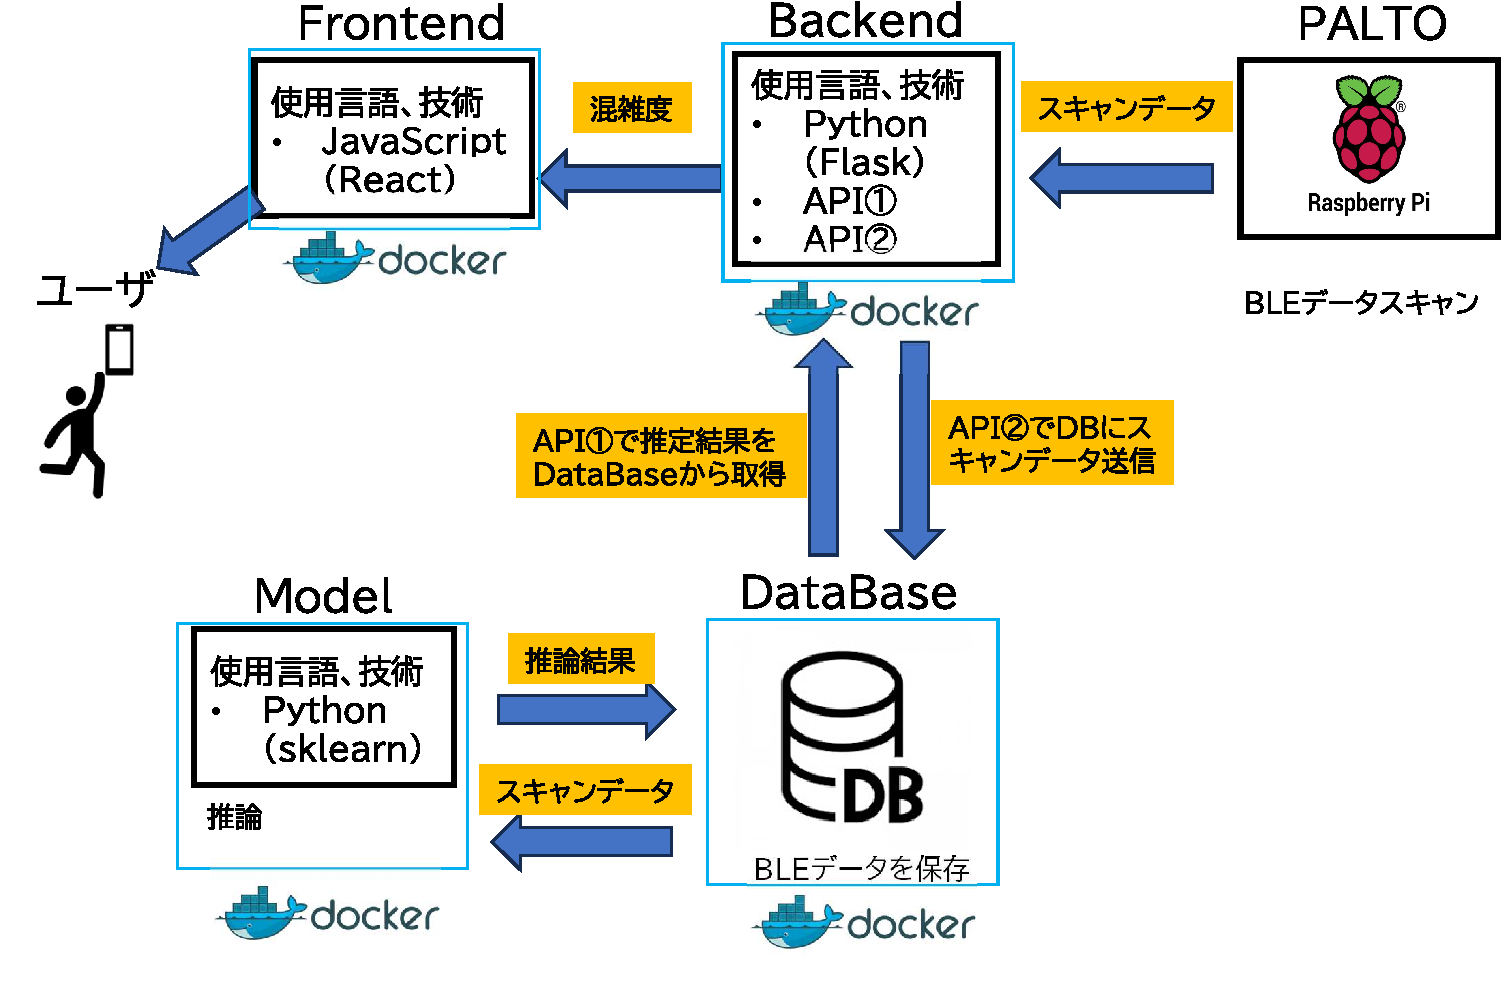
\includegraphics[width=8cm]{./outline_drawing.pdf}
	\caption{システム概要図}
	\label{fig:システム概要図}
\end{figure}

本システムのデータの流れを図\ref{fig:システム概要図}に示し,
以下にその各ステップを説明する.
\begin{enumerate}
	\item データ収集 \\
	Raspberry PiがBLEスキャンを実行し,取得したデータをWi-Fi経由でサーバへ送信する.
	
	\item データ保存 \\
	API\textcircled{2}を通じて,受信したデータをデータベースコンテナに保存する.
	
	\item データ処理・予測 \\
	モデルコンテナがデータベースから取得した最新の1分間のデータから人数を予測し,データベースに保存する.
	
	\item 予測結果の取得・提供 \\
	ユーザーがアプリケーションの更新ボタンを押すと,
	API\textcircled{1}を通じてデータベースコンテナから予測結果を取得し,フロントエンドコンテナへ提供する.
	
	\item データの可視化 \\
	フロントエンドコンテナが取得したデータを可視化し,ユーザーに混雑状況を提供する.
\end{enumerate}

\subsection*{2. フロントエンドの工夫点}

続いて,フロントエンドの工夫点について述べる.

\subsubsection*{(1)Reactの採用}
フロントエンド開発には,JavaScriptライブラリであるReactを採用した.Reactは,以下の点で本システムに適していると判断した.

\begin{itemize}
	\item コンポーネントベースのUI設計
	
	UIをコンポーネント単位で分割して開発することで,コードの再利用性が高まり,メンテナンス性も向上した.また,機能ごとに責務を分離することで,チーム開発における分業が容易になった.
	
	\item 宣言的なパラダイム
	
	手続き型のコードとは異なるシンプルな記述により,コードの可読性が向上した.状態の変化に応じてUIがどのように変化するべきかを宣言的に記述できるため,複雑なDOMの操作を直接行う必要がなくなった.
	
	\item 効率的なレンダリング
	
	仮想DOM(Virtual DOM)の採用により,ブラウザで表示するUIを効率的に(最低限の描画で)レンダリングすることが可能になった.これにより,アプリケーションのパフォーマンスが向上し,ユーザーエクスペリエンスが改善された.
\end{itemize}

\subsubsection*{(2)レスポンシブデザインの実装}
本システムでは,様々なデバイスからのアクセスを想定し,ブラウザで表示するUIをレスポンシブデザインで設計した.これにより,デスクトップPCからスマートフォンまで,異なる画面サイズに対応したユーザーインターフェースを提供することが可能になった.

図\ref{fig:responsive_design}に示すように,デバイスのサイズに応じてレイアウトが自動的に調整され,どのデバイスからもストレスなく操作できる環境を実現した.

% ここに図を入れる場合
% \begin{figure}[tb]
%	\centering
%	\includegraphics[width=0.8\linewidth]{responsive_design.png}
%	\caption{レスポンシブデザインの例}
%	\label{fig:responsive_design}
% \end{figure}

\subsubsection*{(3)動的なUI表現の実装}
本システムでは,ユーザーエクスペリエンスを向上させるため,以下のような動的なUI表現を実装した.

\begin{itemize}
	\item 混雑度表示のアニメーション化
	
	システムが推定した混雑度を,単なる数値や静的なグラフィックではなく,動的なアニメーションで表現することで,より直感的に混雑状況を把握できるようにした.これにより,ユーザーは一目で現在の混雑状況を理解することが可能になった.
	
	\item 更新機能の簡素化
	
	更新ボタンを設計することにより,予測時刻の更新を簡素化した.ユーザーはボタン一つで最新の混雑情報を取得でき,操作の煩雑さを排除することで,ユーザーエクスペリエンスの向上を図った.
	
\end{itemize}

表\ref{tbl:UI_components}に,主要なUIコンポーネントとその役割について示す.

\begin{table}[tb]
	\centering
	\caption{主要なUIコンポーネント}
	\label{tbl:UI_components}
	\small
	\doublerulesep=0.3pt
	\begin{tabular}{l|p{9cm}} \hline\hline\hline
		コンポーネント名 & 役割 \\ \hline
		CongestionDisplay & 混雑度をアニメーションと数値で表示するコンポーネント \\ \hline
		UpdateButton & 最新の予測データを取得するためのボタンコンポーネント \\ \hline
		TimeStampDisplay & 予測時刻を表示するコンポーネント \\ \hline
		ResponsiveContainer & 画面サイズに応じてレイアウトを調整するコンテナコンポーネント \\ \hline\hline\hline
	\end{tabular}
\end{table}
\section*{3. バックエンドの工夫点}
\chapter*{B-3. 開発体制}
\section*{1. プロジェクト全体の体制}
\section*{2. プロジェクト管理・コミュニケーション}

本節では,我々がプロジェクトを円滑に進めるために使用していた管理ツールおよび進捗や問題の報告等を実現するための体制について述べる.
\begin{itemize}
	\item \textbf{プロジェクト管理ツール}
	
	今回のプロジェクトへ取り組むにあたり,IoT 機器による BLE 取得や混雑度を可視化させるシステムの処理内容を記述したソースコードの管理,
	並びにタスクの管理を実現するために以下の 2 つのツールを用いた.
	
	\begin{enumerate}
		\item \textbf{GitHub}
		
		GitHub とは,Git\cite{Git} を基盤とするリポジトリ(データベース)を用いたソースコード管理と開発者同士のコラボレーションを実現するプラットフォームのことである\cite{GitHub}.
%		分散型のソースコード管理では,各開発者がリモートリポジトリとは別にローカルリポジトリを個人のローカルディスクに持ち,
%		ローカルリポジトリに対してコミット等の処理を行う仕組みになっているものをいう(図\ref{fig:分散型のバージョン管理}).
%		なお,そのままでは開発者間でリポジトリを共通できないため,必要に応じてローカルリポジトリの内容とリモートリポジトリの内容を同期させることになる.
%		\begin{figure}[H]
%			\centering
%			\includegraphics[scale=0.6]{./fig/distributed\_vcs.pdf}
%			\caption{分散型のバージョン管理}
%			\label{fig:分散型のバージョン管理}
%		\end{figure}
		
		\item \textbf{Notion}
		
		Notion とは,メモ・タスク管理・ドキュメント作成・データベース機能を統合した多機能な情報管理ツールのことである\cite{Notion}.
		
	\end{enumerate}
	
	\item \textbf{コミュニケーション体制}
	
	進捗確認や課題の報告等を目的として対面の定例ミーティングを週 1 日で実施した.
\end{itemize}


\section*{3. スケジュールとマイルストーン}

  
  \small
  \bibliographystyle{jsai}
  \bibliography{ref}
\end{document}

